\subsection{Numerische Gitter}
\label{sec:num_gitter}

Sind das mathematische Modell mit seinen Differentialgleichungen sowie den nötigen
Rand- sowie gegebenenfalls Anfangsbedingungen festgelegt, besteht der nächste Schritt
bei der Anwendung eines numerischen Berechnungsverfahren darin, das kontinuierliche
Gebiet von Raum und ggf. Zeit durch eine endliche Menge von Teilgebieten zu approximieren,
in denen dann der Wert des gesuchten Größe berechnet wird.

Diese Teilgebiete werden im Allgemeinen in Form eines Gitters über den zu untersuchenden
Bereich $V$ gelegt, weshalb dieser Arbeitsschritt auch oft Gittergenerierung genannt wird.

Ein wichtiges Unterscheidungskriterium ist die Anordnung der Gitterpunkte.
Man unterscheidet grundsätzlich zwischen strukturierten und unstrukturierten Gittern.

Bei strukturierten Gittern ist die Lage der Gitterpunkte zueinander festgelegt. Diese
Lagebeziehungen müssen deshalb nicht aufwendig gespeichert werden und die Gittergenerierung
ist schnell und ohne großen Rechenaufwand nötig. Zwar ist es möglich bestimmte Gebiete
aus der Gittergenerierung auszuschließen, eine Anpassung an die Problemgeometrie ist
jedoch nur innerhalb der vorgegebenen Lagebeziehungen möglich.

Bei unstrukturierten Gittern hingegen gibt es keine Vorschriften zu den Lagebeziehungen
der einzelnen Gitterpunkte. Diese müssen deshalb aufwendig gespeichert werden, was
den Speicherverbrauch sowie die Lösung komplizierter macht. Andererseits ist es problemlos möglich
das Gitter an der Problemgeometrie auszurichten oder in bestimmten Gebieten selektiv zu verfeinern,
sowie die Gittergeneration einfacher zu bewerkstelligen

\subsubsection{Physikalisches und logisches Gebiet}

Oftmals lässt die Geometrie des zu untersuchenden Problems keine Anwendung eines
strukturierten Gitters zu. Nicht in jeden Fall ist es jedoch nötig daraufhin unstrukturierte
Gitter zu verwenden. Vielmehr ist es möglich das physikalische Gebiet des Problems
mittels einer geeigneten mathematischen Transformation auf ein sogenanntes
logisches Gebiet abzubilden, auf welchem dann die Anwendung eines strukturierten Gitters
möglich ist. Exemplarisch ist diese Transformation in Abbildung~\ref{fig:transf} zu sehen.
\begin{figure}[ht]
%\newcommand{\pder}[2][]{\frac{\partial#1}{\partial#2}}
%\newcommand{\pderf}[1]{\frac{\partial f}{\partial#1}}
%\newcommand{\pderfs}[1]{\frac{\partial^2 f}{\partial#1}}

\newcommand{\fxi}{f_{\xi}}
\newcommand{\fxxi}{f_{\xi\xi}}
\newcommand{\fxxxi}{f_{\xi\xi\xi}}
\newcommand{\fxxxxi}{f_{\xi\xi\xi\xi}}
\newcommand{\xxi}{x_{\xi}}
\newcommand{\xxxi}{x_{\xi\xi}}
\newcommand{\xxxxi}{x_{\xi\xi\xi}}
\newcommand{\xxxxxi}{x_{\xi\xi\xi\xi}}
\newcommand{\yxi}{y_{\xi}}
\newcommand{\yxxi}{y_{\xi\xi}}
\newcommand{\yxxxi}{y_{\xi\xi\xi}}
\newcommand{\yxxxxi}{y_{\xi\xi\xi\xi}}

\newcommand{\feta}{f_{\eta}}
\newcommand{\feeta}{f_{\eta\eta}}
\newcommand{\feeeta}{f_{\eta\eta\eta}}
\newcommand{\feeeeta}{f_{\eta\eta\eta\eta}}
\newcommand{\xeta}{x_{\eta}}
\newcommand{\xeeta}{x_{\eta\eta}}
\newcommand{\xeeeta}{x_{\eta\eta\eta}}
\newcommand{\xeeeeta}{x_{\eta\eta\eta\eta}}
\newcommand{\yeta}{y_{\eta}}
\newcommand{\yeeta}{y_{\eta\eta}}
\newcommand{\yeeeta}{y_{\eta\eta\eta}}
\newcommand{\yeeeeta}{y_{\eta\eta\eta\eta}}


\newcommand{\etai}{\eta_{e1}}
\newcommand{\etaii}{\eta_{e2}}
\newcommand{\etilde}{\tilde{e}}


%\chapter{Transformation}

%Die Transformation vom physikalischen auf den logischen Bereich mit
%den physikalischen Koordinaten $(x, y)$ sowie den logischen
%Koordinaten $(\xi, \eta)$ kann wie folgt definiert werden:
%\begin{equation}
  %x=x(\xi,\eta),\quad y=y(\xi, \eta)
%\end{equation}
%\begin{equation}
  %\pder[x]{\xi}=\xi_x=\frac{y_{\eta}}{J}
%\end{equation}
%Damit folgt für für die bei Konvektion und Diffusion auftretende
%erste und zweite Ableitung:

%\begin{align*}
  %\pderf{x}&=\pder[\xi]{x}\pderf{\xi}+\pder[\eta]{x}\pderf{\eta}
  %=\frac{y_{\eta}}{J} f_{\xi} - \frac{y_{\xi}}{J}f_{\eta}\\
  %\pderf{y}&=\pder[\xi]{y}\pderf{\xi}+\pder[\eta]{y}\pderf{\eta}
  %=\frac{x_{\xi}}{J}f_{\eta}-\frac{x_{\eta}}{J} f_{\xi} \\
  %\pderfs{x^2} &= \pder{x}\left({\frac{y_{\eta}}{J} f_{\xi} - \frac{y_{\xi}}{J}f_{\eta}}\right)\\
               %&= \frac{\yeta^2}{J^2} \fxxi + \frac{\yxi^2}{J^2} \feeta-2 \frac{\yxi \yeta}{J^2} f_{\xi\eta}\\
               %&+ \frac{1}{J^3} \Big[\fxi
  %\Big(-2\xxi\yxi\yeta\yeeta + 2\xxi\yeta^2y_{\xi\eta} + \xxxi \yeta^3 - 2x_{\xi \eta}\yxi\yeta^2
  %-\xeta\yeta^2\yxxi + \xeta\yxi^2\yeeta + \yeeta\yxi^2\yeta\Big)\\
  %&+ \feta\Big(
  %2\xeta\yxi\yeta\yxxi - 2\xeta\yxi^2y_{\xi\eta} -\xeeta\yxi^3+2x_{\xi\eta}\yeta\yxi^2
  %+\xxi\yxi^2\yeeta-\xxi\yeta^2\yxxi-\xxxi\yeta^2\yxi
%\Big)\Big]
%\end{align*}


%Im logischen Gebiet können nun die vorhandenen Ableitungen von $f$
%($f_{\xi}$, $f_{\eta}$, $\dots$) diskretisiert werden.
%Es werden hierbei Zentraldifferenzen zweiter Ordnung gewählt.

%\begin{equation}
  %f_{\xi}=\frac{f_{i+1,j}-f_{i-1,j}}{2\Delta \xi} - \frac{f_{\xi\xi\xi}}{6}\Delta \xi^2 + HOT
%\end{equation}
%\begin{equation}
  %f_{\eta}=\frac{f_{i,j+1}-f_{i,j-1}}{2 \Delta \eta} - \frac{f_{\eta\eta\eta}}{6}\Delta \eta^2 + HOT
%\end{equation}
%\begin{equation}
  %\fxxi=\frac{f_{i+1,j}-2f_{i,j}+f_{i-1,j}}{\Delta \xi^2} -\frac{\fxxxxi}{12} \Delta \xi^2 + HOT
%\end{equation}
%\begin{equation}
  %\feeta=\frac{f_{i,j+1}-2f_{i,j}+f_{i,j-1}}{\Delta \eta^2} -\frac{\feeeeta}{12} \Delta \eta^2 + HOT
%\end{equation}
%\begin{equation}
  %f_{\xi\eta}=\frac{f_{i+1,j+1}-2f_{i,j}+f_{i-1,j-1}}{\Delta \xi\Delta \eta} -\frac{\fxxi+\feeta}{4} \Delta \eta \Delta \xi + HOT
%\end{equation}

%Werden diese nun eingesetzt ergibt sich für $\Delta \xi = 1$ folgende Form:

%\begin{equation}
  %\pderf{x}=\frac{y_{\eta}}{J}\frac{f_{i+1,j}-f_{i-1,j}}{2}
  %- \frac{y_{\xi}}{J}\frac{f_{i,j+1}-f_{i,j-1}}{2}
%\end{equation}

%sowie der entstehende Abbruchfehler:

%\begin{equation}
  %TE_x = -\frac{y_{\eta}}{J}\frac{f_{\xi\xi\xi}}{6}
  %+ \frac{y_{\xi}}{J}\frac{f_{\eta\eta\eta}}{6}+HOT
%\end{equation}

%Anschließend können die berechneten Werte für $f_{\xi},\dots$
%eingesetzt werden.

%\begin{align*}
  %\fxi &= \xxi f_x + \yxi f_y\\
  %\fxxi &= \xxxi f_x + \xxi^2f_{xx}+2\xxi \yxi f_{xy}
  %+\yxi^2 f_{yy} + \yxxi f_y\\
  %\fxxxi &= \xxxxi f_x + \yxxxi f_y + 3 \xxxi\xxi f_{xx}+
  %3 \yxxi\yxi f_{yy} + \left({3\xxxi\yxi+3\yxxi\xxi}\right)f_{xy}\\
  %&+ \xxi^3f_{xxx}+\yxi^3f_{yyy}+3\xxi^2\yxi f_{xxy}+3\xxi\yxi^2f_{xyy}\\
 %\feeeta &= \xeeeta f_x + \yeeeta f_y + 3 \xeeta\xeta f_{xx}+
  %3 \yeeta\yeta f_{yy} + \left({3\xeeta\yeta+3\yeeta\xeta}\right)f_{xy}\\
  %&+ \xeta^3f_{xxx}+\yeta^3f_{yyy}+3\xeta^2\yeta f_{xxy}+3\xeta\yeta^2f_{xyy}
%\end{align*}

%Es ergibt sich:

%\begin{align*}
  %TE_x&= -\frac{y_{\eta}}{J} \frac{1}{6}\Big[\xxxxi f_x + \yxxxi f_y + 3 \xxxi\xxi f_{xx}+
  %3 \yxxi\yxi f_{yy} + \left({3\xxxi\yxi+3\yxxi\xxi}\right)f_{xy}\\
%&+ \xxi^3f_{xxx}+\yxi^3f_{yyy}+3\xxi^2\yxi f_{xxy}+3\xxi\yxi^2f_{xyy}\Big]\\
%&+  \frac{y_{\xi}}{J}\frac{1}{6} \Big[\xeeeta f_x + \yeeeta f_y + 3 \xeeta\xeta f_{xx}+
  %3 \yeeta\yeta f_{yy} + \left({3\xeeta\yeta+3\yeeta\xeta}\right)f_{xy}\\
  %&+ \xeta^3f_{xxx}+\yeta^3f_{yyy}+3\xeta^2\yeta f_{xxy}+3\xeta\yeta^2f_{xyy}
%\Big]\\
  %&= TE_{x1} + TE_{x2} + TE_{x3}
%\end{align*}

%wobei $TE_{x1}$die ersten Ableitungen von $f$ enthält, usw.:

%\begin{align*}
  %TE_{x1} &= \frac{1}{6\ J}\left[{
  %\left({-\yeta\xxxxi + \yxi\xeeeta}\right) f_x +
  %\left({-\yeta\yxxxi + \yxi\yeeeta}\right) f_y
  %}\right]\\
  %TE_{x2} &= \frac{1}{2\ J} \Big[
  %\left({-\yeta\xxxi\xxi + \yxi\xeeta\xeta}\right) f_{xx}+
  %\left({-\yeta\yxxi\yxi + \yxi\yeeta\yeta}\right) f_{yy}\\&+
  %\left({-\yeta \left({\xxxi\yxi+\yxxi\xxi}\right) +
  %\yxi \left({\xeeta\yeta+\yeeta\xeta}\right)}\right) f_{xy}
  %\Big]\\
  %TE_{x3}&=\frac{1}{6\ J} \Big[
  %\left({-\yeta\xxi^3+\yxi\xeta^3}\right) f_{xxx}+
  %\yxi \yeta\left({-\yxi^2+\yeta^2}\right) f_{yyy}\\&+
  %3 \yxi \yeta \left({-\xxi^2+\xeta^2}\right) f_{xxy}+
  %3 \yxi \yeta \left({-\xxi\yxi+\xeta\yeta}\right) f_{xyy}
  %\Big]
%\end{align*}




\section{Abbruchfehler für nicht-orthogonale Gitter}

Bei der Verwendung von orthogonalen Gittern vereinfachen sich viele Terme oder
heben sich mit der Gegenseite auf. Diese müssen im Falle eines nicht-orthogonalen
numerischen Gitters beachtet werden, soll die Berechnung realistische Werte liefern.

Da viele der zusätzlichen Terme auf der Verzerrtheit des Gitters beruhen und eine
Betrachtung im physikalischen Bereich verkomplizieren, wird eine Transformation auf
den logischen Bereich durchgeführt. Der Vorteil besteht darin, dass auf dem dortigen kartesischen
Gitter die Anwendung von Differenzenschemata einfach ist und man die zusätzlichen Fehler des
verzerrten Gitters vermeiden kann. Der Nachteil ist die zusätzliche Komplexität durch
die Transformation. Die Transformation eines Kontrollvolumens vom physikalischen in
den logischen Bereich ist in Abbildung~\ref{fig:no-trans} dargestellt.
\begin{figure}[ht]
  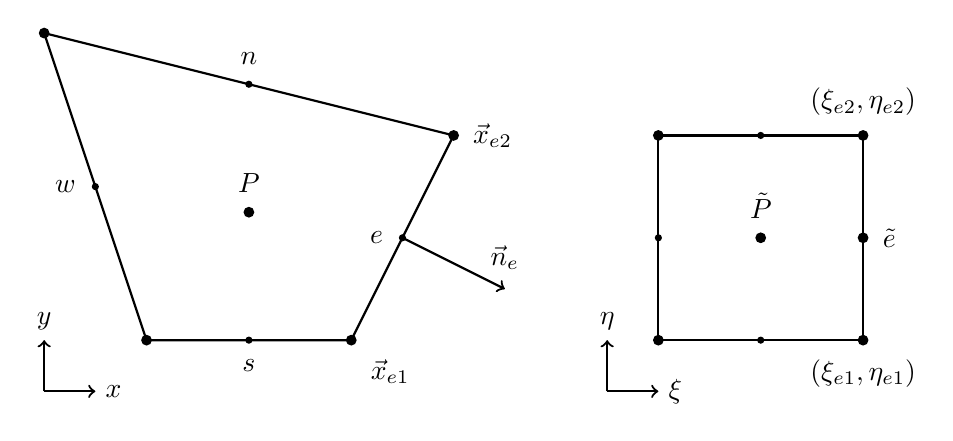
\begin{tikzpicture}[scale=1.3]
  \draw[->, thick] (-1,-0.5) -- (-0.5,-0.5) node[right] {$x$} coordinate(x axis);
  \draw[->, thick] (-1,-0.5) -- (-1,0) node[above] {$y$} coordinate(y axis);

  \draw[thick] (0,0) -- (2,0) -- (3,2) -- (-1, 3) --cycle;
  \fill (1,1.25) circle[radius=1.5pt];
  \node (x) at (1,1.25) [label=above:$P$] {};
  \fill (2,0) circle[radius=1.5pt];
  \node (x) at (2,0) [label=below right:$\vec x_{e1}$] {};
  \fill (3,2) circle[radius=1.5pt];
  \node (x) at (3,2) [label=right:$\vec x_{e2}$] {};

  \fill (-1,3) circle[radius=1.5pt];
  \fill (0,0) circle[radius=1.5pt];

  \fill (1,0) circle[radius=1pt];
  \node (x) at (1,0) [label=below:$s$] {};
  \fill (2.5,1) circle[radius=1pt];
  \node (x) at (2.5,1) [label=left:$e$] {};
  \fill (1,2.5) circle[radius=1pt];
  \node (x) at (1,2.5) [label=above:$n$] {};
  \fill (-0.5,1.5) circle[radius=1pt];
  \node (x) at (-0.5,1.5) [label=left:$w$] {};


  \draw[->, thick] (2.5,1) -> (3.5,0.5);
  \node (x) at (3.5,0.5) [label=above:$\vec n_e$] {};



  % xi-eta
  \draw[->, thick] (4.5,-0.5) -- (5,-0.5) node[right] {$\xi$} coordinate(x axis);
  \draw[->, thick] (4.5,-0.5) -- (4.5,0) node[above] {$\eta$} coordinate(y axis);

  \draw[thick] (5, 0) rectangle (7, 2);
  \fill (7, 1)  circle[radius=1.5pt];
  \node (x) at (7,1) [label={right}:{$\tilde{e}$}] {};

  \fill (5, 0)  circle[radius=1.5pt];
  \fill (5, 2)  circle[radius=1.5pt];
  \fill (5, 1)  circle[radius=1pt];
  \fill (6, 2)  circle[radius=1pt];
  \fill (6, 0)  circle[radius=1pt];

  \fill (7, 0)  circle[radius=1.5pt];
  \node (x) at (7,0) [label=below:{$(\xi_{e1},\eta_{e1})$}] {};
  \fill (7, 2)  circle[radius=1.5pt];
  \node (x) at (7,2) [label=above:{$(\xi_{e2}, \eta_{e2})$}] {};

  \fill (6, 1)  circle[radius=1.5pt];
  \node (x) at (6,1) [label=above:{$\tilde{P}$}] {};
\end{tikzpicture}

\centering
\caption{Transformation eines Kontrollvolumens}
\label{fig:no-trans}
\end{figure}

\noindent Die Ableitung des Abbruchfehlers soll hier beispielhaft an der östlichen Seite des Kontrollvolumens
gezeigt werden. Bei einer Transportgleichung mit konvektivem und diffusivem Term entsteht damit folgendes
Integral:
\begin{equation}
  \int_{\mathbf{x}_{e1}}^{\mathbf{x}_{e2}}\left({\rho v_i\phi+\alpha \pder[\phi]{x_i}}\right)n_{ei}ds
  \label{eq:int_trans}
\end{equation}
Hierbei bezeichnen $\mathbf{x}_{e1}$ und $\mathbf{x}_{e2}$ Anfangs- und Endpunkt, sowie $\mathbf{n}_e$
den Einheitsnormalenvektor der Ostseite, wie in Abbildung~\ref{fig:no-trans} gezeigt.
Statt der direkten Auswertung erfolgt nun die Transformation ins logische Gebiet. Dazu wird die
Transformationsregel eines Wegintegrals genutzt.
\begin{equation}
  \int_{\gamma}f\ ds=\int_a^bf(\gamma (t)) \lVert \dot{\gamma}(t)\rVert_2 dt
\end{equation}
Bei der Koordinatentransformation ergibt sich, dass der Wert von $\xi$ auf der Ostseite konstant sein muss.
Die Transformation von Gleichung~\eqref{eq:int_trans} ergibt:
\begin{align*}
  \underbrace{
    \int_{\eta_{e1}}^{\eta_{e2}} \left({\rho v_1 \phi n_{e1}}\right)
  \left\lVert \frac{\partial x(\xi=e, \eta)}{\partial \eta} \right\rVert_2 d\eta
  }_I
  &+ \underbrace{
  \int_{\eta_{e1}}^{\eta_{e2}} \left({\alpha \pder[\phi]{x} n_{e1}}\right)
  \left\lVert \frac{\partial x(\xi=e, \eta)}{\partial \eta} \right\rVert_2 d\eta
}_{II}\\
  + \underbrace{
  \int_{\eta_{e1}}^{\eta_{e2}} (\rho v_2 \phi n_{e2})
  \left\lVert \frac{\partial x(\xi=e, \eta)}{\partial \eta} \right\rVert_2 d\eta
  }_{III}
  &+ \underbrace{
  \int_{\eta_{e1}}^{\eta_{e2}} \left({\alpha \pder[\phi]{x} n_{e2}}\right)
  \left\lVert \frac{\partial x(\xi=e, \eta)}{\partial \eta} \right\rVert_2 d\eta
  }_{IV}
\end{align*}
Hierbei beschreiben die Terme $I$ und $III$ die konvektiven Flüsse, die Terme $II$ und $IV$ sind
diffusive Flüsse. Bei $III$ und $IV$ handelt es sich um Terme, die auf orthogonalen Gittern wegfallen würden,
da hier die zweite Komponente des Einheitsnormalenvektors Null wäre.
Im Folgenden werden nun wieder Abbruchfehler der einzelnen Terme abgeleitet. Bei den Flüssen muss dabei
einerseits der Abbruchfehler der Integralapproximation über die Mittelpunktsregel ermittelt werden.
Andererseits muss der Abbruchfehler aus der Fluss- bzw. Ableitungsapproximation ermittelt werden.



\paragraph{Konvektive Terme}

\noindent
Bei Integration mit der Mittelpunktsregel folgt für Term $I$:
\begin{equation*}
  C=(\rho v_1 \phi n_{e1})
  \left\lVert \frac{\partial x(\xi=e, \eta)}{\partial \eta} \right\rVert_2
\end{equation*}

\begin{align*}
  I&= C\big\vert_{\tilde{e}} \underbrace{(\etaii-\etai)}_{=1} + \frac{1}{2} \pder[C]{\eta}\bigg\vert_{\tilde{e}}
  \underbrace{\left({(\etaii-\etilde)^2-(\etai-\etilde)^2}\right)}_{=0}
  +\frac{1}{6} \frac{\partial^2 C}{\partial \eta^2}\bigg\vert_{\tilde{e}}
  \underbrace{\left({(\etaii-\etilde)^3-(\etai-\etilde)^3}\right)}_{=\frac{1}{4}} + HOT\\
  &= C \big\vert_{\tilde{e}}+ \underbrace{\frac{1}{24}  \frac{\partial^2 C}{\partial \eta^2}
\bigg\vert_{\tilde{e}}+HOT}_{TE_{C,\,int,\,e}}
\end{align*}
Hierbei wird die Abkürzung $C$ zur Übersichtlichkeit eingeführt und $\tilde{e}$ bezeichnet den Mittelpunkt
der transformierten Ostseite (siehe Abbildung~\ref{fig:no-trans}).  Nach dem allgemeinen Vorgehen bei der
Methode der Finiten Volumen muss nun $C\vert_{\tilde{e}}$ durch die umgebenden Zellenmittelpunkte ausgedrückt werden.
Dies soll hier mit dem Zentraldifferenzenschema gezeigt werden.
\begin{align*}
   C\big\vert_{\tilde{e}}
   =& C\big\vert_{\tilde{E}}
   \left({\frac{\xi_{\tilde{e}}-\xi_{\tilde{P}}}{\xi_{\tilde{E}}-\xi_{\tilde{P}}}}\right)
   + C\big\vert_{\tilde{P}} \left({1-\frac{\xi_{\tilde{e}}-\xi_{\tilde{P}}}{\xi_{\tilde{E}}-\xi_{\tilde{P}}} }\right)
   + \frac{1}{2} \frac{\partial^2 C}{\partial \xi^2}\bigg\vert_{\tilde{P}}
   (\xi_{\tilde{e}}-\xi_{\tilde{E}})(\xi_{\tilde{e}}-\xi_{\tilde{P}})\\
   &+ \frac{1}{6}  \frac{\partial^3 C}{\partial \xi^3}\bigg\vert_{\tilde{P}}
   \left({(\xi_{\tilde{e}}-\xi_{\tilde{P}})^2-(\xi_{\tilde{E}}-\xi_{\tilde{P}})^2}\right)
   (\xi_{\tilde{e}}-\xi_{\tilde{P}}) + HOT\\
   =&\frac{1}{2} C \big\vert_{\tilde{E}} + \frac{1}{2} C \big\vert_{\tilde{P}}
   \underbrace{- \frac{1}{8} \frac{\partial^2 C}{\partial \xi^2}\bigg\vert_{\tilde{P}}
   - \frac{1}{16} \frac{\partial^3 C}{\partial \xi^3}\bigg\vert_{\tilde{P}} + HOT}_{TE_{CDS,\,e}}
\end{align*}



\paragraph{Diffusive Terme}
\noindent
Bei Term $II$ wird ebenfalls die Mittelpunktsregel angewandt. Mit der Abkürzung $D$
ergibt sich hier:
\begin{equation*}
  D=  \left({\alpha \pder[\phi]{x} n_{e1}}\right)
  \left\lVert \frac{\partial x(\xi=e, \eta)}{\partial \eta} \right\rVert_2 d\eta
\end{equation*}

\begin{align*}
  II&= D\big\vert_{\tilde{e}} \underbrace{(\etaii-\etai)}_{=1} + \frac{1}{2}
  \frac{\partial^2 D}{\partial \eta^2} \bigg\vert_{\tilde{e}}
  \underbrace{\left({(\etaii-\etilde)^2-(\etai-\etilde)^2}\right)}_{=0}
  +\frac{1}{6} \frac{\partial^3 D}{\partial \eta^3}\bigg\vert_{\tilde{e}}
  \underbrace{\left({(\etaii-\etilde)^3-(\etai-\etilde)^3}\right)}_{=\frac{1}{4}} + HOT\\
  &= D \big\vert_{\tilde{e}}+ \underbrace{\frac{1}{24}  \frac{\partial^3 D}{\partial \eta^3}
\bigg\vert_{\tilde{e}}+HOT}_{TE_{D,\,int,\,e}}
\end{align*}
Hier muss nun beachtet werden, dass $D$ selbst noch die Ableitung $\pder[\phi]{x}$ im physikalischen Gebiet enthält.
Diese muss wie das Kontrollvolumen ins logische Gebiet transformiert werden. Die Transformation ergibt
mit der Jakobimatrix aus Gleichung~\eqref{eq:detj} für
die Ableitung $\pder[\phi]{x}$:% und $\pder[\phi]{y}$:
\begin{align}
  \pder[\phi]{x}&=\pder[\xi]{x}\pder[\phi]{\xi}+\pder[\eta]{x}\pder[\phi]{\eta}
  = \frac{\yeta}{det(J)} \phi_{\xi} - \frac{\yxi}{det(J)} \phi_{\eta}
\end{align}
  %\pder[\phi]{y}&=\pder[\xi]{y}\pderf{\xi}+\pder[\eta]{y}\pderf{\eta}
  %=\frac{x_{\xi}}{det(J)}\phi_{\eta}-\frac{x_{\eta}}{det(J)} \phi_{\xi}
%\end{align}

Bei der anschließenden Approximation von $D_{\tilde{e}}$ durch die Mittelpunkte der Nachbarkontrollvolumen
muss ebenfalls die $\frac{\partial \phi}{\partial x}$ transformiert werden. Damit ergibt sich folgende Gleichung:



%\begin{equation}
  %D =\left({\frac{\alpha\ n_{e1}}{det\ J}}\right)
  %\left\lVert \frac{\partial x(\xi=e, \eta)}{\partial \eta} \right\rVert_2 
%\left({\yeta(\phi_{\tilde{E}}-\phi_{\tilde{P}}) - \yxi(\phi_{\tilde{ne}}-\phi_{\tilde{se}})}\right)
%\end{equation}

\begin{align*}
  D\big\vert_{\etilde} &=
  \left({\frac{\alpha\ n_{e1}}{det\ J}}\right)
  \left\lVert \frac{\partial x(\xi=e, \eta)}{\partial \eta} \right\rVert_2 
  \Bigg(\yeta(\phi_{\tilde{E}}-\phi_{\tilde{P}}) - \yxi(\phi_{\tilde{ne}}-\phi_{\tilde{se}})
      \underbrace{ -\frac{\yeta}{6} \frac{\partial^3 \phi}{\partial \xi^3} \bigg\vert_{\etilde}
      +\frac{\yeta}{6} \frac{\partial^3 \phi}{\partial \xi^3} \bigg\vert_{\etilde}
+ HOT}_{TE_{D,\,e}}\Bigg)
\end{align*}
Auch $\phi_{\tilde{ne}}$ und $\phi_{\tilde{se}}$ müssen durch die umliegenden Zellenwerte ausgedrückt werden.
Dies kann beispielsweise durch lineare Interpolation erfolgen.
\begin{equation}
\phi_{\tilde{ne}} = \frac{\phi_{\tilde{P}} +\phi_{\tilde{E}} + \phi_{\tilde{NE}}+ \phi_{\tilde{N}}}{4} 
\end{equation}

In der oben stehenden Gleichung treten auch $\yxi$ und $\yeta$ auf. Diese werden Metriken der Transformation genannt und
sind nur vom Gitter, nicht aber von der Lösungsfunktion abhängig. Ihre Approximation
wird in Abschnitt~\ref{sec:verz-metrik} gezeigt.





\paragraph{Quellterm}
\noindent
Zur Berechnung des Abbruchfehlers des Quellterms von nicht-orthogonalen Gittern wird der Transformationssatz benötigt.
Dieser lautet im zweidimensionalen Fall:
\begin{equation}
  \int \int_A f(x,y)\ dx\,dy = \int \int_P f\left({x(\xi,\,\eta),\ y(\xi,\,\eta)}\right)\ det(J)\ d\xi\,d\eta
\end{equation}
Angewandt auf den Quellterm und der Abkürzung $Q$ ergibt sich für den Quellterm:
\begin{equation}
  \begin{IEEEeqnarraybox}[][c]{rCl}
    \int\int_{P} \underbrace{\Pi_{\phi}(\xi, \eta) det(J) }_{Q} d\xi d\eta
    &=& Q\big\vert_{\tilde{P}} (\xi_e-\xi_w)(\eta_n-\eta_s)\\
  & &+ Q_{\xi}\big\vert_{\tilde{P}} \frac{(\xi_e-\xi_P)^2 - (\xi_w-\xi_P)^2}{2} (\eta_n-\eta_s)\\
  && + Q_{\eta}\big\vert_{\tilde{P}} \frac{(\eta_n-\eta_P)^2-(\eta_s-\eta_P)^2}{2} (\xi_e-\xi_w) \\
  & &+ \frac{1}{2} Q_{\xi\xi}\big\vert_{\tilde{P}}\frac{(\xi_e-\xi_P)^3 - (\xi_w-\xi_P)^3}{3} (\eta_n-\eta_s)\\
  &&+ \frac{1}{2} Q_{\eta\eta}\big\vert_{\tilde{P}} \frac{(\eta_n-\eta_P)^3-(\eta_s-\eta_P)^3}{3} (\xi_e-\xi_w) \\
  & &+ Q_{\xi\eta}\big\vert_{\tilde{P}} \frac{(\xi_e-\xi_P)^2 - (\xi_w-\xi_P)^2}{2} \cdot
  \frac{(\eta_n-\eta_P)^2-(\eta_s-\eta_P)^2}{2} + HOT\\
  &=&Q\big\vert_{\tilde{P}} + \underbrace{\frac{1}{24} \left({Q_{\xi\xi}\big\vert_{\tilde{P}}+Q_{\eta\eta}\big\vert_{\tilde{P}}}\right)
+ HOT}_{TE_{Q}}
\end{IEEEeqnarraybox}
\end{equation}
Die gezeigten Ableitungen müssen nun für die anderen Seiten des Kontrollvolumens wiederholt werden.
Anschließend werden sie summiert und ergeben dann den Abbruchfehler eines Kontrollvolumens auf
einem nicht-orthogonalem Gitter.





\subsection{Diskretisierung der Metriken}
\label{sec:verz-metrik}

In den oben gezeigten Ableitungen treten mehrfach Größen auf, die nur vom numerischen Gitter, nicht aber
von der Lösungsfunktion abhängen. Diese werden Metriken genannt.
Meistens handelt es sich hierbei um physikalische Variablen, die nach logischen Koordinaten abgeleitet werden.
Beispiele sind $x_{\xi}$ oder $y_{\eta\eta}$.

Metriken sind analytische Größen und müssen im Rahmen der Berechnung diskretisiert werden.
Treten die Metriken bei einer Approximation über die Grenzen des Kontrollvolumens auf,
ist die Diskretisierung verschieden zur Approximation innerhalb der Grenzen eines Kontrollvolumens.

\paragraph{Diskretisierung innerhalb eines Kontrollvolumens}
\begin{figure}[ht]
  \begin{tikzpicture}[scale=1.2]
  \draw[->, thick] (-2,0) -- (-1.5,0) node[right] {$x$} coordinate(x axis);
  \draw[->, thick] (-2,0) -- (-2,0.5) node[above] {$y$} coordinate(y axis);

  \fill[tud0a] (0,0) -- (3,0.5) -- (3.5,3.5) -- (0.5, 3) --cycle;

  \draw[thick] (-0.5,-0.08333) -- (4,0.66666);
  \draw[thick] (-0.08333,-0.5) -- (0.66666,4);
  \draw[thick] (-0.5,-0.16666+3) -- (4.5,3.66666);
  \draw[thick] (-.08333+3,0) -- (0.5833+3,4);

  \draw[thick,<->] (15mm,0mm) arc (0:9.5:15mm);
  \draw[thick,<->] (0mm,15mm) arc (90:80.5:15mm);
  \draw[thick,<->] (9mm,1.5mm) arc (9.5:81:9mm);

  \node (x) at (1.5,0.05) [label=below:$\gamma$]{};
  \node (x) at (0.05,1.5) [label=left:$\beta$]{};
  \node (x) at (0.5,0.5) [label=above right:$\theta$]{};

  \node (x) at (2.5,0.3) [label=above left:$a$]{};
  \node (x) at (0.3,2.5) [label=below right:$b$]{};

  %\node (x) at (4,0.66666) [label=right:{$\eta=j-\frac{1}{2}$}]{};
  %\node (x) at (4.5,3.66666) [label=right:{$\eta=j+\frac{1}{2}$}]{};
  %\node (x) at (0.66666,4) [label=left:{$\xi=i-\frac{1}{2}$}]{};
  %\node (x) at (0.66666+3,4) [label=left:{$\xi=i+\frac{1}{2}$}]{};

  \draw[thick] (0,0) -- (2,0);
  \draw[thick] (0,0) -- (0,2);
\end{tikzpicture}

\centering
\caption{Größen für die Berechnung der Metriken innerhalb des Kontrollvolumens}
\end{figure}

\noindent
Die Metriken innerhalb eines Kontrollvolumens sind beispielsweise für die Transformation
des Quellterms nötig. Zur Diskretisierung der Metriken werden
Differenzenquotienten als Approximationen genutzt \cite{lee}.
Beispielsweise ergibt sich auf einem zweidimensionalen nicht-orthogonalen
Gitter mit $\Delta\xi = \Delta \eta = 1$:
\begin{equation}
  x_{\xi} = \frac{x_{i+1, j} - x_{i-1,j}}{\Delta \xi} = x_{i+1, j} - x_{i-1,j} = a \cos \gamma
\end{equation}
Für die anderen Metriken erster Ordnung ergeben sich:
\begin{align*}
  x_{\eta} &= b\sin \beta\\
  y_{\xi} &= a \sin \gamma\\
  y_{\eta} &= b \cos \beta
\end{align*}
Eine weitere benötige Größe stellt die Determinante der Jakobimatrix
dar. Sie ist für jedes Kon\-troll\-volumen unterschiedlich. Werden
die diskretisierten Metriken eingesetzt ergibt sich folgende Gleichung:
\begin{align}
  det(J) &= x_{\xi}y_{\eta}-x_{\eta}y_{\xi}\nonumber\\
    &= a \cos \gamma \, b \cos \beta - 
       a \sin \beta \, b \sin \gamma\nonumber\\
       &= ab(\cos\gamma\cos\beta-\sin\beta\sin\gamma)
\end{align}
Hier kann nun das folgende Additionstheorem
angewendet werden.
\begin{equation*}
\cos(\beta+\gamma)=\cos\gamma\cos\beta-\sin\beta\sin\gamma
\end{equation*}
Da weiterhin bekannt ist, dass $\beta+\gamma
+\theta = 90^{\circ}$ ist, ergibt sich mit der Beziehung
$\sin(x)=\cos(\frac{\pi}{2} -x)$ letztendlich aus
Gleichung~\eqref{eq:detj} der folgende Term für $J$. Er stellt den Betrag des
Kreuzprodukts der beiden
Vektoren dar,
die das Kontrollvolumen aufspannen.
Es handelt sich somit um eine Approximation des Flächeninhalts
des Kontrollvolumens.
\begin{equation}
  det(J) = a b \sin \theta
\end{equation}

\paragraph{Diskretisierung über Kontrollvolumengrenzen}

\noindent
Bei der Approximation der diffusiven und konvektiven Flüsse werden meist
auch die Grenzen eines Kontrollvolumens überschritten. Damit kommt auch
die Geometrie des Nachbarkontrollvolumens zum Tragen und die Diskretisierung der
Metriken muss angepasst werden.
\begin{figure}[ht]
  \begin{tikzpicture}[scale=1.5]
  \draw[->, thick] (-1.5,0) -- (-1,0) node[right] {$x$} coordinate(x axis);
  \draw[->, thick] (-1.5,0) -- (-1.5,0.5) node[above] {$y$} coordinate(y axis);

  \fill[tud0a] (0,1) -- (2,0.5) -- (2.5,2) -- (0.5, 3) --cycle;
  \draw[thick] (0,1) -- (2,0.5) -- (2.5,2) -- (0.5, 3) --cycle;
  \draw[thick] (4,-0.5) -- (2,0.5) -- (2.5,2) -- (5, 2.5) --cycle;

  \fill (2,0.5,0) circle[radius=1.5pt];
  \node (x) at (2,0.5) [label=below left:$se$] {};
  \fill (2.5,2) circle[radius=1.5pt];
  \node (x) at (2.5,2) [label=below right:$ne$] {};
  \fill (1.25,1.625) circle[radius=1.5pt];
  \node (x) at (1.25,1.625) [label=above:$P$] {};
  \node (x) at (1.25,1.625) [label=below:{$(\xi_{i,j},\ \eta_{i,j})$}] {};
  \fill (3.25,1.125) circle[radius=1.5pt];
  \node (x) at (3.25,1.125) [label=above:$E$] {};
  \node (x) at (3.25,1.125) [label=below:{$(\xi_{i+1,j},\ \eta_{i+1,j})$}] {};

  \draw[thick,->] (-0.75,2.125) -- (5.25,0.625);
  \node (x) at (5.25,0.625) [label=right:$\xi$] {};

  \draw[thick,->] (1.75,-0.25) -- (2.75,2.75);
  \node (x) at (2.75,2.75) [label=right:$\eta$] {};
\end{tikzpicture}

\centering
\caption{Berechnung der Metriken über Grenzen von Kontrollvolumen}
\end{figure}

Die Ableitungen nach $\xi$ werden nach folgendem Schema approximiert, wobei
$\vert \mathbf{x}_E -\mathbf{x}_P \vert$ den Abstand der Punkte $E$ und $P$ beschreibt.
\begin{equation}
  \pder[x]{\xi} \approx \frac{x_E-x_P}{\vert \mathbf{x}_E -\mathbf{x}_P \vert} \qquad
  \text{und} \qquad \pder[y]{\xi} \approx \frac{y_E-y_P}{\vert \mathbf{x}_E -\mathbf{x}_P \vert}
\end{equation}
Die Ableitungen nach $\eta$ ergeben sich mit der Seitenlänge $\delta S_e$ der Ostseite
zu:
\begin{equation}
  \pder[x]{\eta} \approx \frac{x_{ne}-x_{se}}{\delta S_e} \qquad
  \text{und} \qquad \pder[y]{\eta} \approx \frac{y_{ne}-y_{se}}{\delta S_e}
\end{equation}

\centering
\caption{Transformation vom physikalischen ins logische Gebiet}
\label{fig:transf}
\end{figure}
Die Abbildung von physikalischem ($\Omega_p$) auf logisches Gebiet ($\Omega_c$) muss dabei umkehrbar sein, das heißt
die Abbildungsfunktion muss bijektiv sein. Formaler lässt sich die Transformation
$\Omega_c \rightarrow \Omega_p$ wie folgt ausdrücken:
\begin{equation}
  (x,y) = (x(\xi, \eta), y(\xi, \eta)) \quad bzw. \quad (\xi,\eta) = (\xi(x, y), \eta(x,y))
\end{equation}
Hierbei sind $\xi$ und $\eta$ Variablen im logischen Bereich. Sie nehmen diskrete, im allgemeinen äquidistante,
Werte an. Bei $x$ und $y$ handelt es sich um die üblicherweise unregelmäßigen Variablen des physikalischen Bereichs.

Die Jakobimatrix der Transformation stellt einen wichtigen Indikator der Gittereigenschaften dar.
Da die Transformation bijektiv sein muss, darf die Determinante der Jakobimatrix nicht Null werden.
\begin{equation}
  J = 
  \begin{pmatrix}
    \frac{\partial x}{\partial \xi} & \frac{\partial x}{\partial \eta} \\
    \frac{\partial y}{\partial \xi} & \frac{\partial y}{\partial \eta}
  \end{pmatrix}
  \quad und \quad
  det (J) = x_{\xi}y_{\eta} - x_{\eta} y_{\xi} \neq 0
\end{equation}
Die Ableitungen der pysikalischen nach logischen Koordinaten wie
zum Beispiel $x_{\xi}$ werden Metriken genannt. Sie beschrieben Eigenschaften
des Gitters und sind damit nicht lösungsabhängig. Sie existieren auch
für höhere Ableitungen, beispielsweise $x_{\xi\xi}$ oder $y_{\eta\eta}$.
